\documentclass[10pt,a4paper]{article}
\usepackage[margin=22mm]{geometry}
\usepackage[T1]{fontenc}
\usepackage{lmodern,amsmath,amssymb,graphicx,booktabs,microtype}
\usepackage[font=small,labelfont=bf]{caption}
\usepackage[hidelinks]{hyperref}
\usepackage{fancyhdr}
\pagestyle{fancy}\fancyhf{}
\fancyhead[L]{\small Computational Mechanics Projects}
\fancyhead[R]{\small MeshBeacon}
\fancyfoot[C]{\thepage}
\setlength{\headheight}{14pt}
\setlength{\parindent}{0pt}\setlength{\parskip}{5pt}
\setlength{\emergencystretch}{1em}
\newcommand{\R}{\mathbb{R}}
\title{\vspace{-1.3cm}\LARGE MeshBeacon: Residual-Driven Mesh Adaptation for a Localized Elliptic Load}
\author{\small Computational Mechanics Projects\\\small Reproducible technical research note}
\date{\small 29 September 2026}
\begin{document}\maketitle\thispagestyle{fancy}

\begin{abstract}
Uniform refinement can waste degrees of freedom when an elliptic solution has localized gradients. MeshBeacon implements one-dimensional piecewise-linear finite elements, a cell-residual/flux-jump estimator, bulk marking, and nested bisection. An analytical localized solution allows direct comparison against uniform meshes with equal cell counts. The recorded adaptive run uses 426 elements and attains energy error 0.02551, versus 0.16420 on the equal-cell uniform mesh, a ratio of 0.15536. Independent sine refinement recovers second-order $L^2$ and first-order energy convergence. The estimator is explicitly uncalibrated, and quadrature sensitivity is tested rather than assumed away.
\end{abstract}
\section{Introduction}
Adaptive finite elements allocate resolution from the computed solution instead of a prescribed uniform spacing. The practical question is whether residual information identifies where extra elements improve accuracy under a fixed discrete budget. Bulk marking follows the principle introduced by D\"orfler~\cite{dorfler}; this one-dimensional implementation does not inherit the cited two-dimensional theorem automatically. The project emphasizes the complete solve--estimate--mark--refine loop, transparent stopping reasons, and independently evaluated error.
\section{Boundary-value problem}
On the nondimensional interval $(0,1)$, constant diffusion or axial rigidity $a>0$ gives
\begin{equation}
-a u''=f,\qquad u(0)=g_0,\quad u(1)=g_1.
\end{equation}
With homogeneous test functions, the weak form is $\int_0^1au'v'\,dx=\int_0^1fv\,dx$. On an element of length $h_e$, using local coordinate $t\in[0,1]$,
\begin{equation}
K_e=\frac{a}{h_e}\begin{bmatrix}1&-1\\-1&1\end{bmatrix},\qquad
b_e=\int_e f(x)\begin{bmatrix}1-t\\t\end{bmatrix}dx.
\end{equation}
Eliminating prescribed endpoint values includes their right-hand-side correction. The resulting tridiagonal system is solved by a LAPACK banded solver through SciPy. At fixed quadrature order, assembly and one solve use linear work and storage.

For the localized manufactured case, define $b(x)=\exp[-((x-c)/\sigma)^2]$ and
\begin{equation}
u(x)=b(x)-(1-x)b(0)-xb(1),\quad f=-ab'',\quad c=0.37,\quad\sigma=0.04.
\end{equation}
This construction satisfies homogeneous endpoint conditions exactly. Signed loads are intentional. The analytical derivative gives the energy-error norm $\|u-u_h\|_E^2=\int_0^1a(u'-u_h')^2dx$, evaluated independently of the residual estimator.
\newpage
\section{Estimator and adaptive algorithm}
Cell fluxes are $q_e=a(u_{e+1}-u_e)/h_e$. At an interior node the jump is $J_i=q_i-q_{i-1}$. The implemented squared local indicator is
\begin{equation}
\eta_e^2=\frac{h_e^2}{a}\int_e f^2dx+
\frac{h_e}{2a}\sum_{i\in\partial e\cap(0,1)}J_i^2,
\qquad \eta=\left(\sum_e\eta_e^2\right)^{1/2}.
\end{equation}
There is no endpoint jump term under the chosen Dirichlet conditions. Because the piecewise-linear solution has zero cellwise second derivative, the element residual reduces to $f$. The indicator is an uncalibrated estimator, not a proved upper error bound with constant one.

After each solve, squared indicators are sorted in descending order, with ties broken by cell index. The smallest prefix satisfying $\sum_{e\in\mathcal M}\eta_e^2\ge\theta\sum_e\eta_e^2$ is marked, and its cells are bisected. Existing nodes are preserved. In one dimension, nested bisection requires no additional conformity closure. If the entire marked set exceeds the cell budget, refinement is rejected and the last solved state is returned; reaching a resource limit is not reported as convergence.

Python implements the numerical API and experiment logic using compiled NumPy/SciPy primitives. Immutable solver arrays protect mesh/state consistency. Eight-point Gauss--Legendre quadrature assembles the load and estimator; errors use an independent 16-point rule. Public functions separate mesh validation, solving, marking, refinement, and adaptive orchestration.
\section{Validation and recorded evidence}
The adaptive experiment starts with eight cells, $a=1$, bulk fraction $\theta=0.5$, and absolute estimator target 0.15. Uniform comparison solves use exactly the adaptive cell counts. A separate sine solution measures asymptotic convergence.
\begin{center}\begin{tabular}{lr}\toprule
Diagnostic & Recorded value\\\midrule
Adaptive solves / final elements & 22 / 426\\
Adaptive energy error & 0.0255096\\
Equal-cell uniform energy error & 0.1642010\\
Adaptive/uniform error ratio & 0.155356\\
Final estimator / effectivity & 0.125076 / 4.90308\\
Finest sine $L^2$ / energy order & 1.99999 / 0.99999\\\bottomrule
\end{tabular}\end{center}
Changing assembly quadrature from 8 to 16 points changes nodal values by at most $7.03\times10^{-9}$; changing error quadrature from 16 to 24 points changes the measured energy error by $2.64\times10^{-16}$. Patch tests, closed-form quadratic errors, a hand-computed estimator, diffusion scaling, and marking/budget tests provide independent checks beyond the showcase.
Figure~\ref{fig:results} visualizes selected recorded diagnostics.
\newpage
\begin{figure}[!ht]\centering
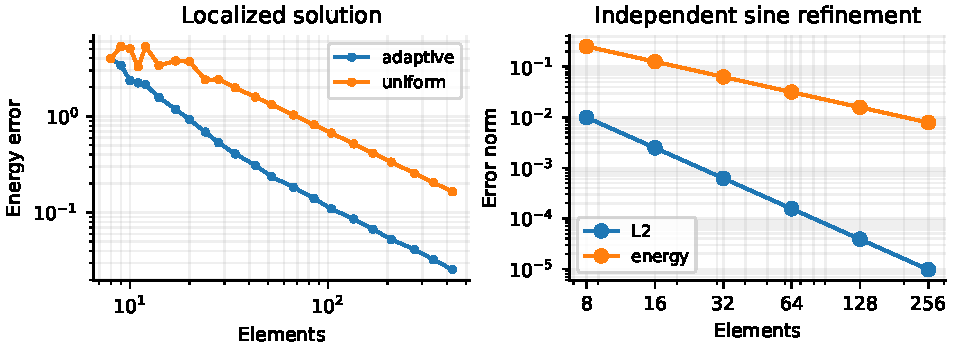
\includegraphics[width=\textwidth]{figure.pdf}
\caption{Recorded error versus element count for the localized solution and independent sine refinement. The adaptive/uniform comparison concerns discrete budget, not runtime.}\label{fig:results}\end{figure}
\section{Discussion and limitations}
Adaptation reduces the energy error substantially at equal final cell count for this localized solution. This is an accuracy-per-degree-of-freedom result, not a runtime speedup: adaptation performs 22 solves and retains a history. The effectivity around 4.90 demonstrates that the raw estimator is conservative for this example, without establishing a universal bound.

A load narrower than mesh and quadrature resolution can be missed by both the solution and estimator. The reported quadrature comparison is evidence for this case, not a universal detection mechanism. The method covers a unit interval, constant diffusion, linear static physics, and two Dirichlet endpoints only. It does not support interfaces, coarsening, multidimensional meshes, or nonlinear laws. Strong grading can cause conditioning problems; numerical error integrals are not interval-certified bounds.
\section{Reproducibility and conclusion}
This note documents the committed implementation at \texttt{751dfa46bd66} and the existing synthetic results; it does not assert new solver runs. Install from the repository root with \texttt{python -m pip install ".[dev]"}; the README gives compiler requirements and verification commands. Code, data, and this manuscript are available at \href{https://github.com/racostacme-come/meshbeacon}{the project repository}. No private course material is reproduced. The manuscript was prepared with AI assistance under the project owner\textquotesingle s direction; no peer review is claimed.
Run \texttt{meshbeacon --output out}; read \texttt{convergence.csv}, \texttt{adaptive\_nodes.csv}, and \texttt{validation.json}. The experiment shows how residual-driven resolution can outperform uniform placement while making the distinction between estimator tolerance, actual error, and resource termination explicit.
\begin{thebibliography}{9}
\bibitem{dorfler} W. D\"orfler, A convergent adaptive algorithm for Poisson's equation, \emph{SIAM J. Numer. Anal.} 33(3), 1106--1124 (1996). \href{https://doi.org/10.1137/0733054}{doi:10.1137/0733054}.
\bibitem{skfem} scikit-fem, \emph{Example 22: adaptive Poisson equation}. \href{https://scikit-fem.readthedocs.io/en/latest/listofexamples.html#example-22-adaptive-poisson-equation}{Online example}; conceptual context for residual and jump indicators.
\end{thebibliography}

\end{document}
